\section{Gruppe} \label{sec:arch_group}
Arkitekturen for gruppe-funktionaliteter er lavet på baggrund af de US, som er opstillet i afsnit \ref{sec:US}. Det er ikke alle US, som er blevet kigget på, og derfor er det kun følgende funktionaliteter, som der er arbejdet på:
\begin{itemize}
    \item Opret gruppe    
    \item Valg af gruppenavn
    \item Tilføjelse/fjernelse af brugere
    \item Tilføje/fjerne administrator rettigheder
    \item Mulighed for at forlade gruppe
    \item Mulighed for at slette gruppe
    \item Mulighed for at tilføje kælenavnetil medlemmer
    \item Mulighed for at videregive owner rettigheder
\end{itemize}

\noindent Der lægges mest vægt på arkitekturen for US’en "Tilføje/fjerne administrator rettigheder", da denne gennemgås igennem rapporten. \\

\subsection{Data view}
I dette view vises der et ER diagram, som beskriver, hvordan data for grupper og dens medlemmer gemmes i databasen. For en detaljeret beskrivelse af, hvordan der er fundet frem til det følgende ER diagramet på figur \ref{fig:group_ER}, henvises der til bilagene. \thomas{Indset henvisning}.
\thomas{Ret diagram}
\begin{figure}[H]
  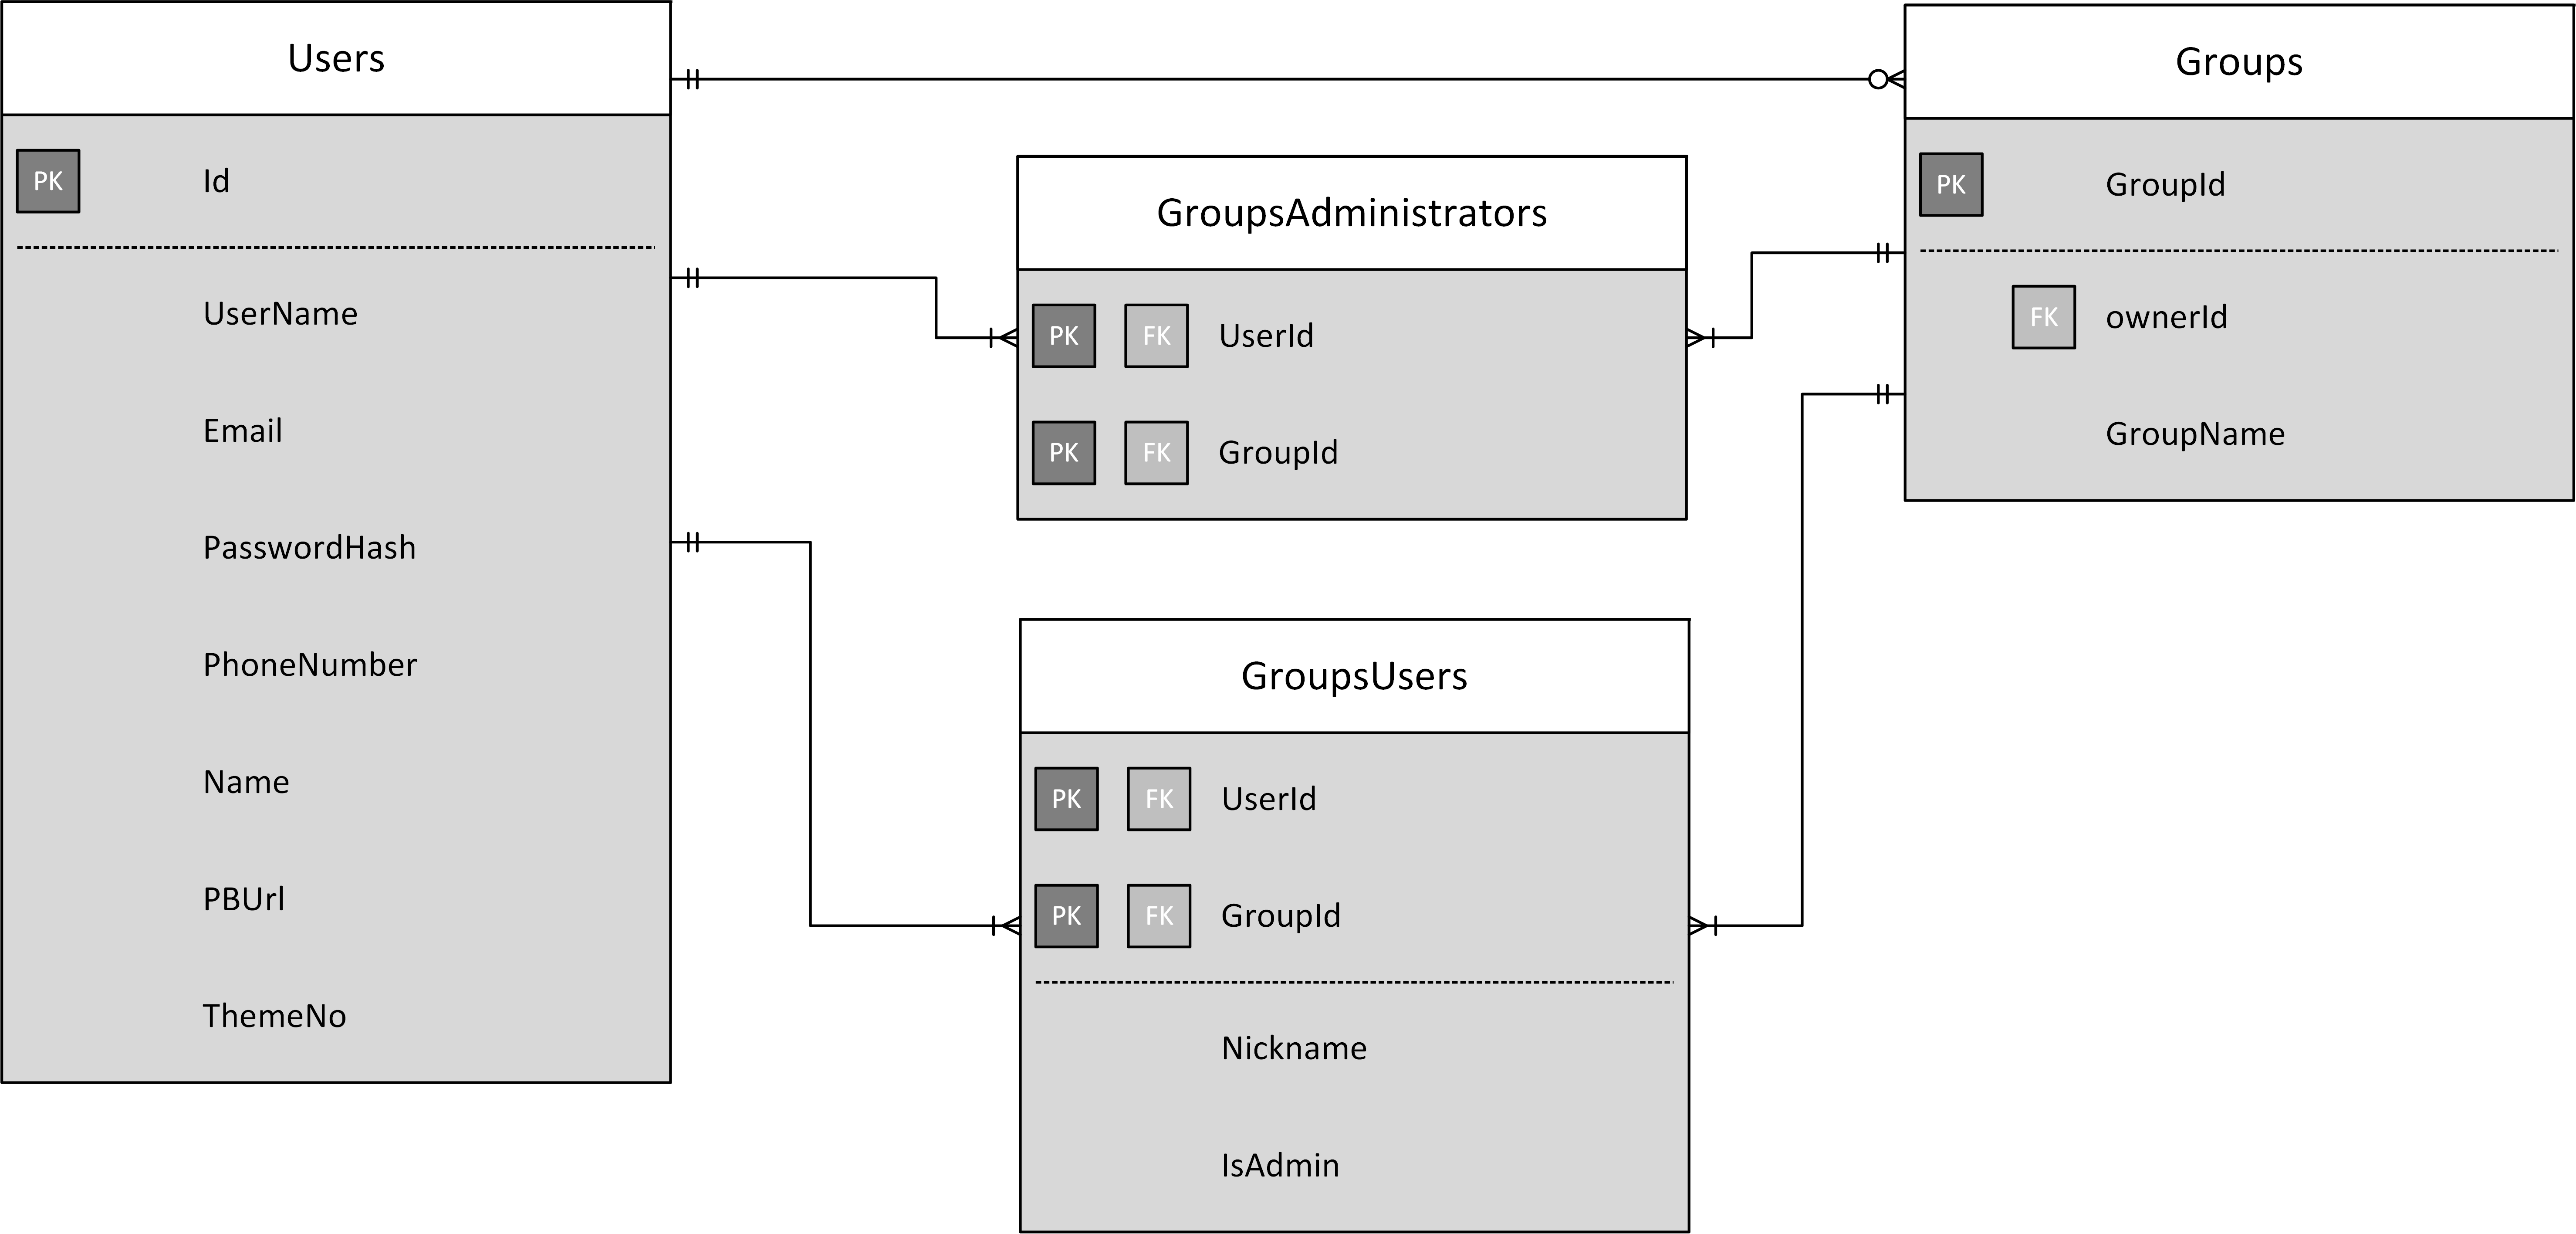
\includegraphics[width=\linewidth]{01_Billeder/09_Arkitektur/Group/Data_Group.png}
  \centering
  \caption{ER Diagram af Groups. Måden det er lavet på, gør at det er muligt at gemme grupper, og deres medlemmer og adminstratorer. Sent i projektet blev det opdaget at tabellen GroupsAdministrators godt kan virke overflødig.}
  \label{fig:group_ER}
\end{figure}

\jonathan{Ændrer rækkefølge på argumenter for GroupAdmins, så det positive ved entiteten kommer først - vidste ikke lige hvordan jeg skulle skrive det.}
\noindent Overflødigheden af GroupAdministrators skyldes at der i GroupsUsers bliver gemt information om hvorvidt et medlem er administrator eller ej. Derfor er der ingen grund til at gemme denne information igen i en anden tabel, da det også bruger plads i databasen. Fordelen ved tabellen er dog at det er hurtigere at finde frem til gruppens administratorer. \\

\subsection{Logical view}
I dette view udarbejdes en controller og views, så US’s til grupper kan blive realiseret. Her bliver det kun vist, hvordan arkitekturen for US’en "Tilføje/fjerne administrator rettigheder" laves, og resten kan findes i bilag. \thomas{indsæt henvisning} \\

\noindent Ideen er, at hjemmesiden skal være nem at bruge, og at der ikke skal navigeres rundt i for mange sider. Derfor er mange af indstillingerne til gruppen skrevet ind i det samme view, herunder US’en "Tilføje/fjerne administrator rettigheder", og der skal være nem adgang til dette view.

\begin{figure}[H]
  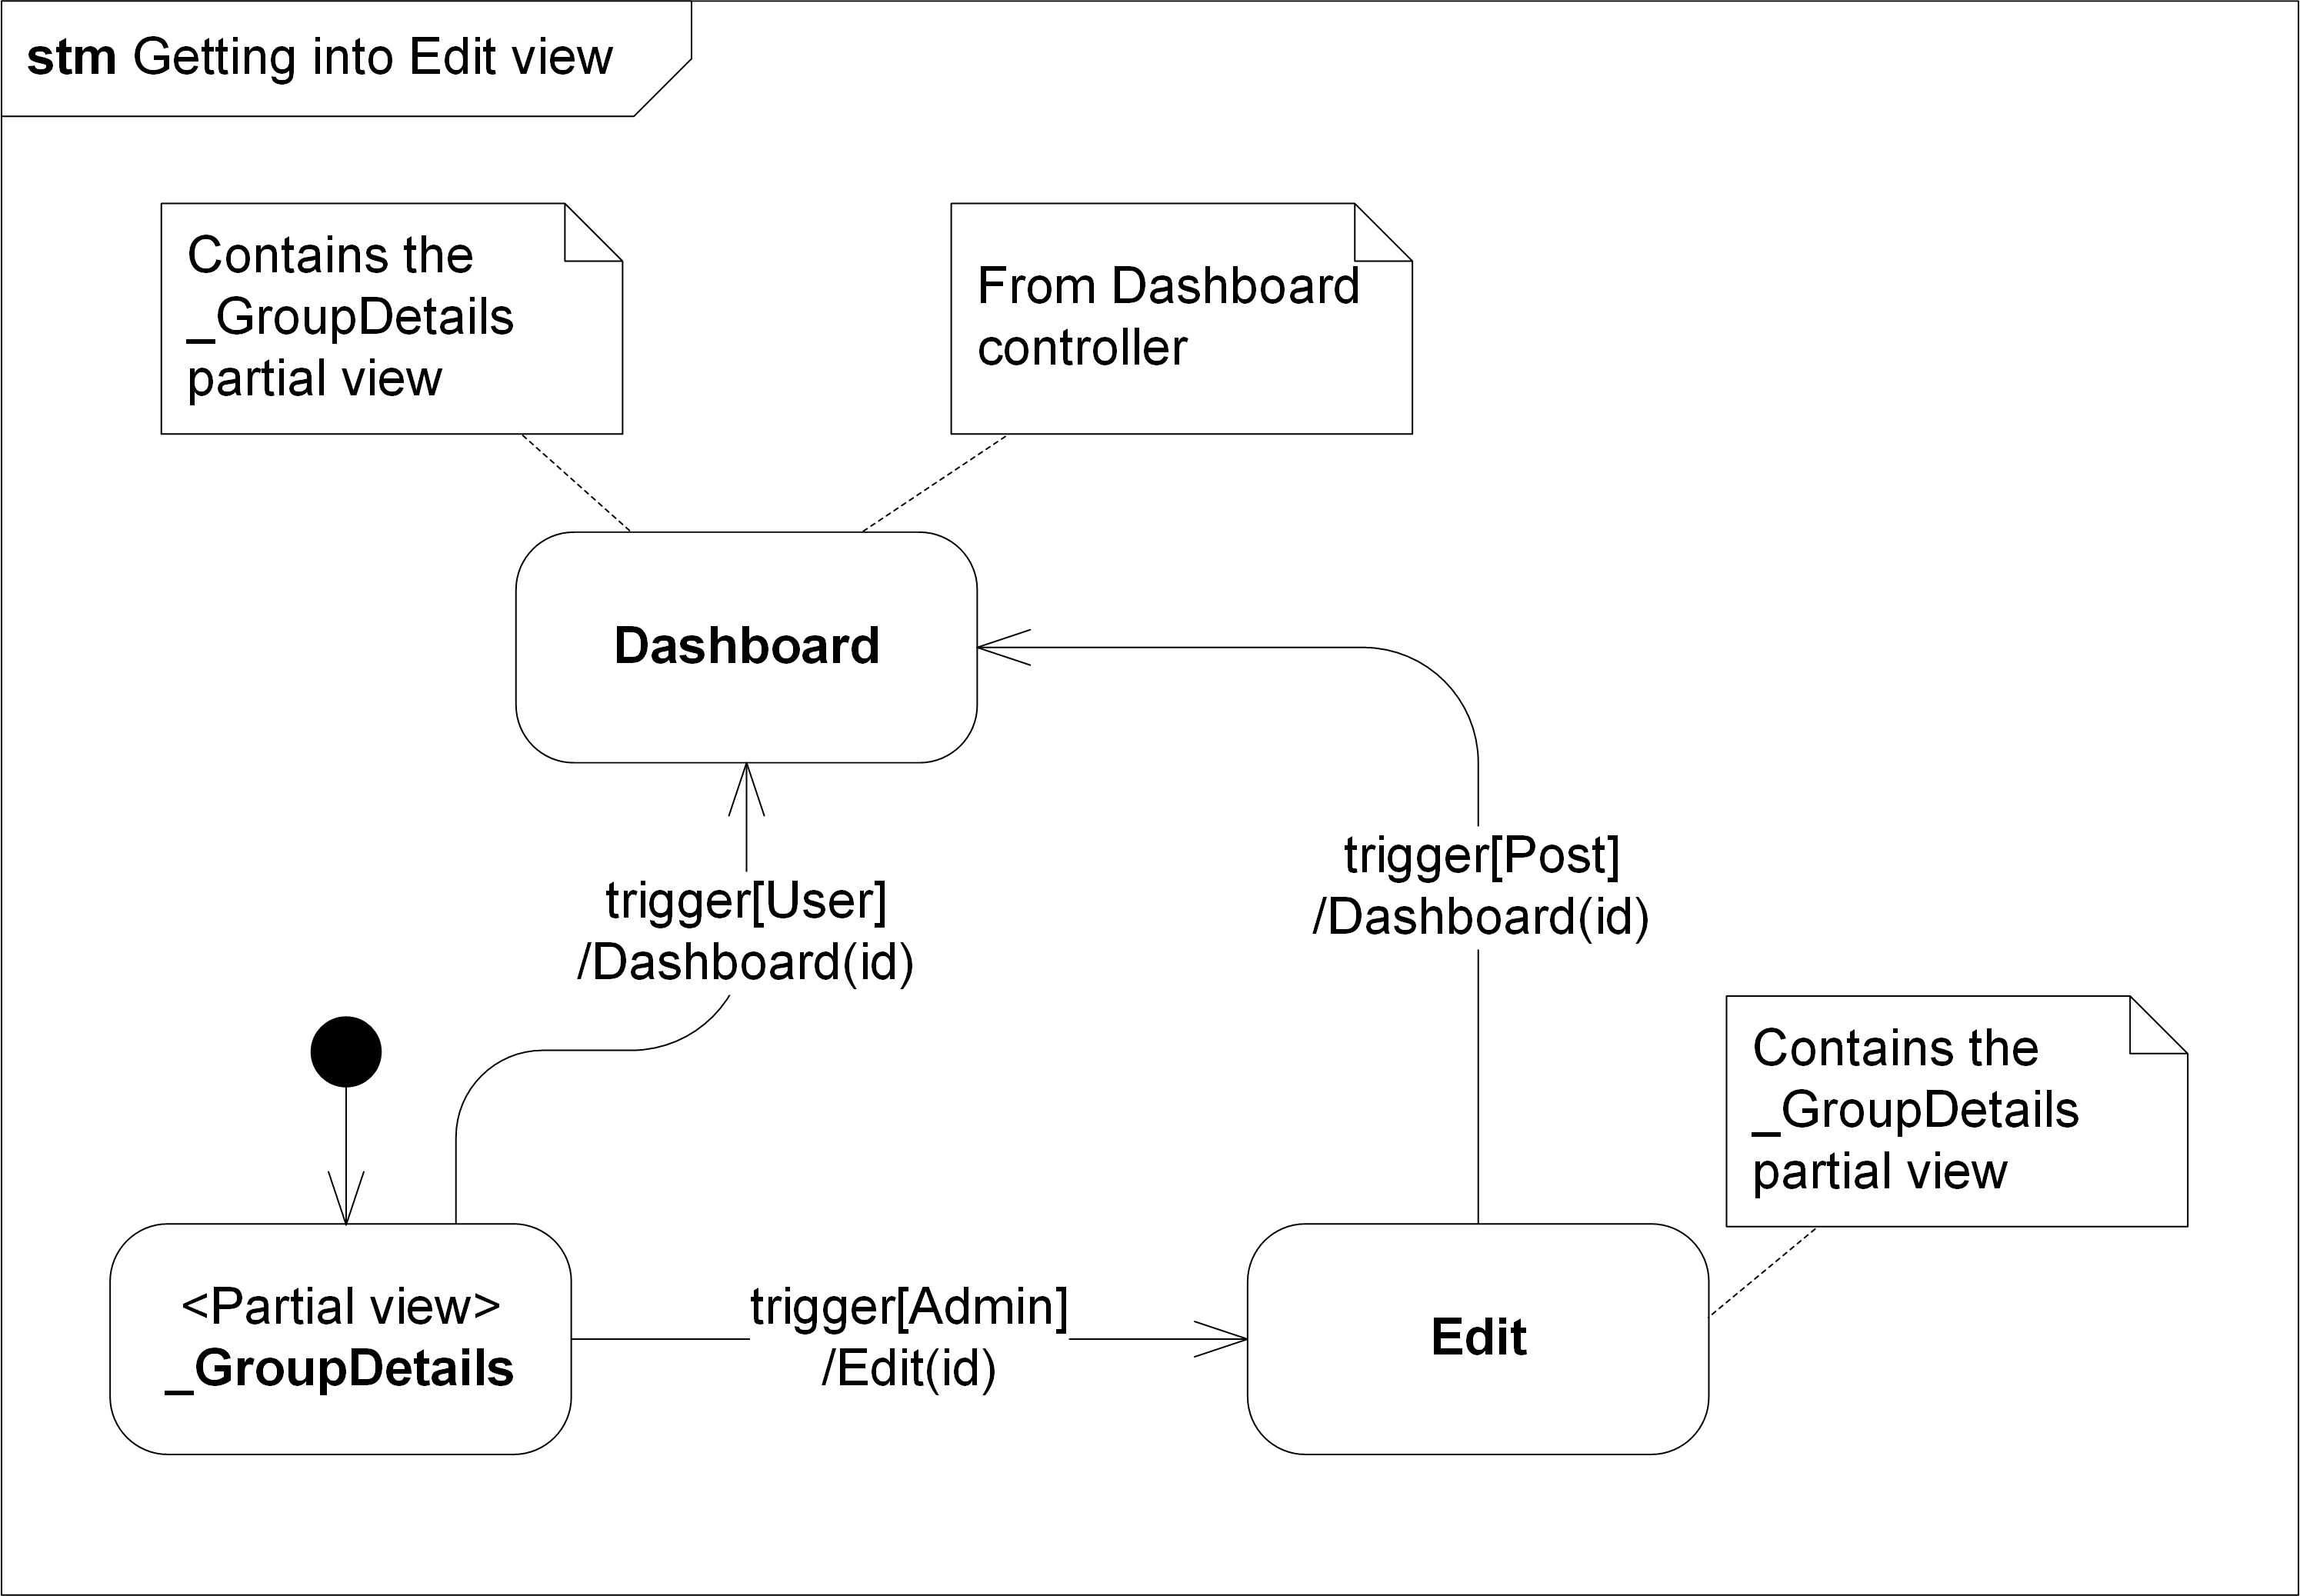
\includegraphics[width=\linewidth]{01_Billeder/09_Arkitektur/Group/LogicalView_Add_Remove_Admin.png}
  \centering
  \caption{Statemachine diagram som viser hvordan man kommer ind i Edit viewet fra \_GroupDetails. Både Edit viewet og Dashboard viewet indeholder \_GroupDetails viewet, og man kan derfor det samme i Edit og Dashboard, som man kan i \_GroupDetails.}
  \label{fig:group_add_remove_admin}
\end{figure}

På figur \ref{fig:group_add_remove_admin} ses Edit viewet, som er viewet, hvor alle gruppens indstillinger kan findes. Herinde skal det være muligt at markere om et medlem er administrator eller ej, ved at markering i en checkboks. Statusen på checkboksen sendes videre til Edit's post funktion, som sørger for at gemme eventuelle ændringer i databasen. På figuren ses der nogle funktionskald mellem de forskellige views. Disse skal skrives ind i klassen GroupController, som kan ses på figur \ref{fig:group_logical_class}.

\begin{figure}[H]
  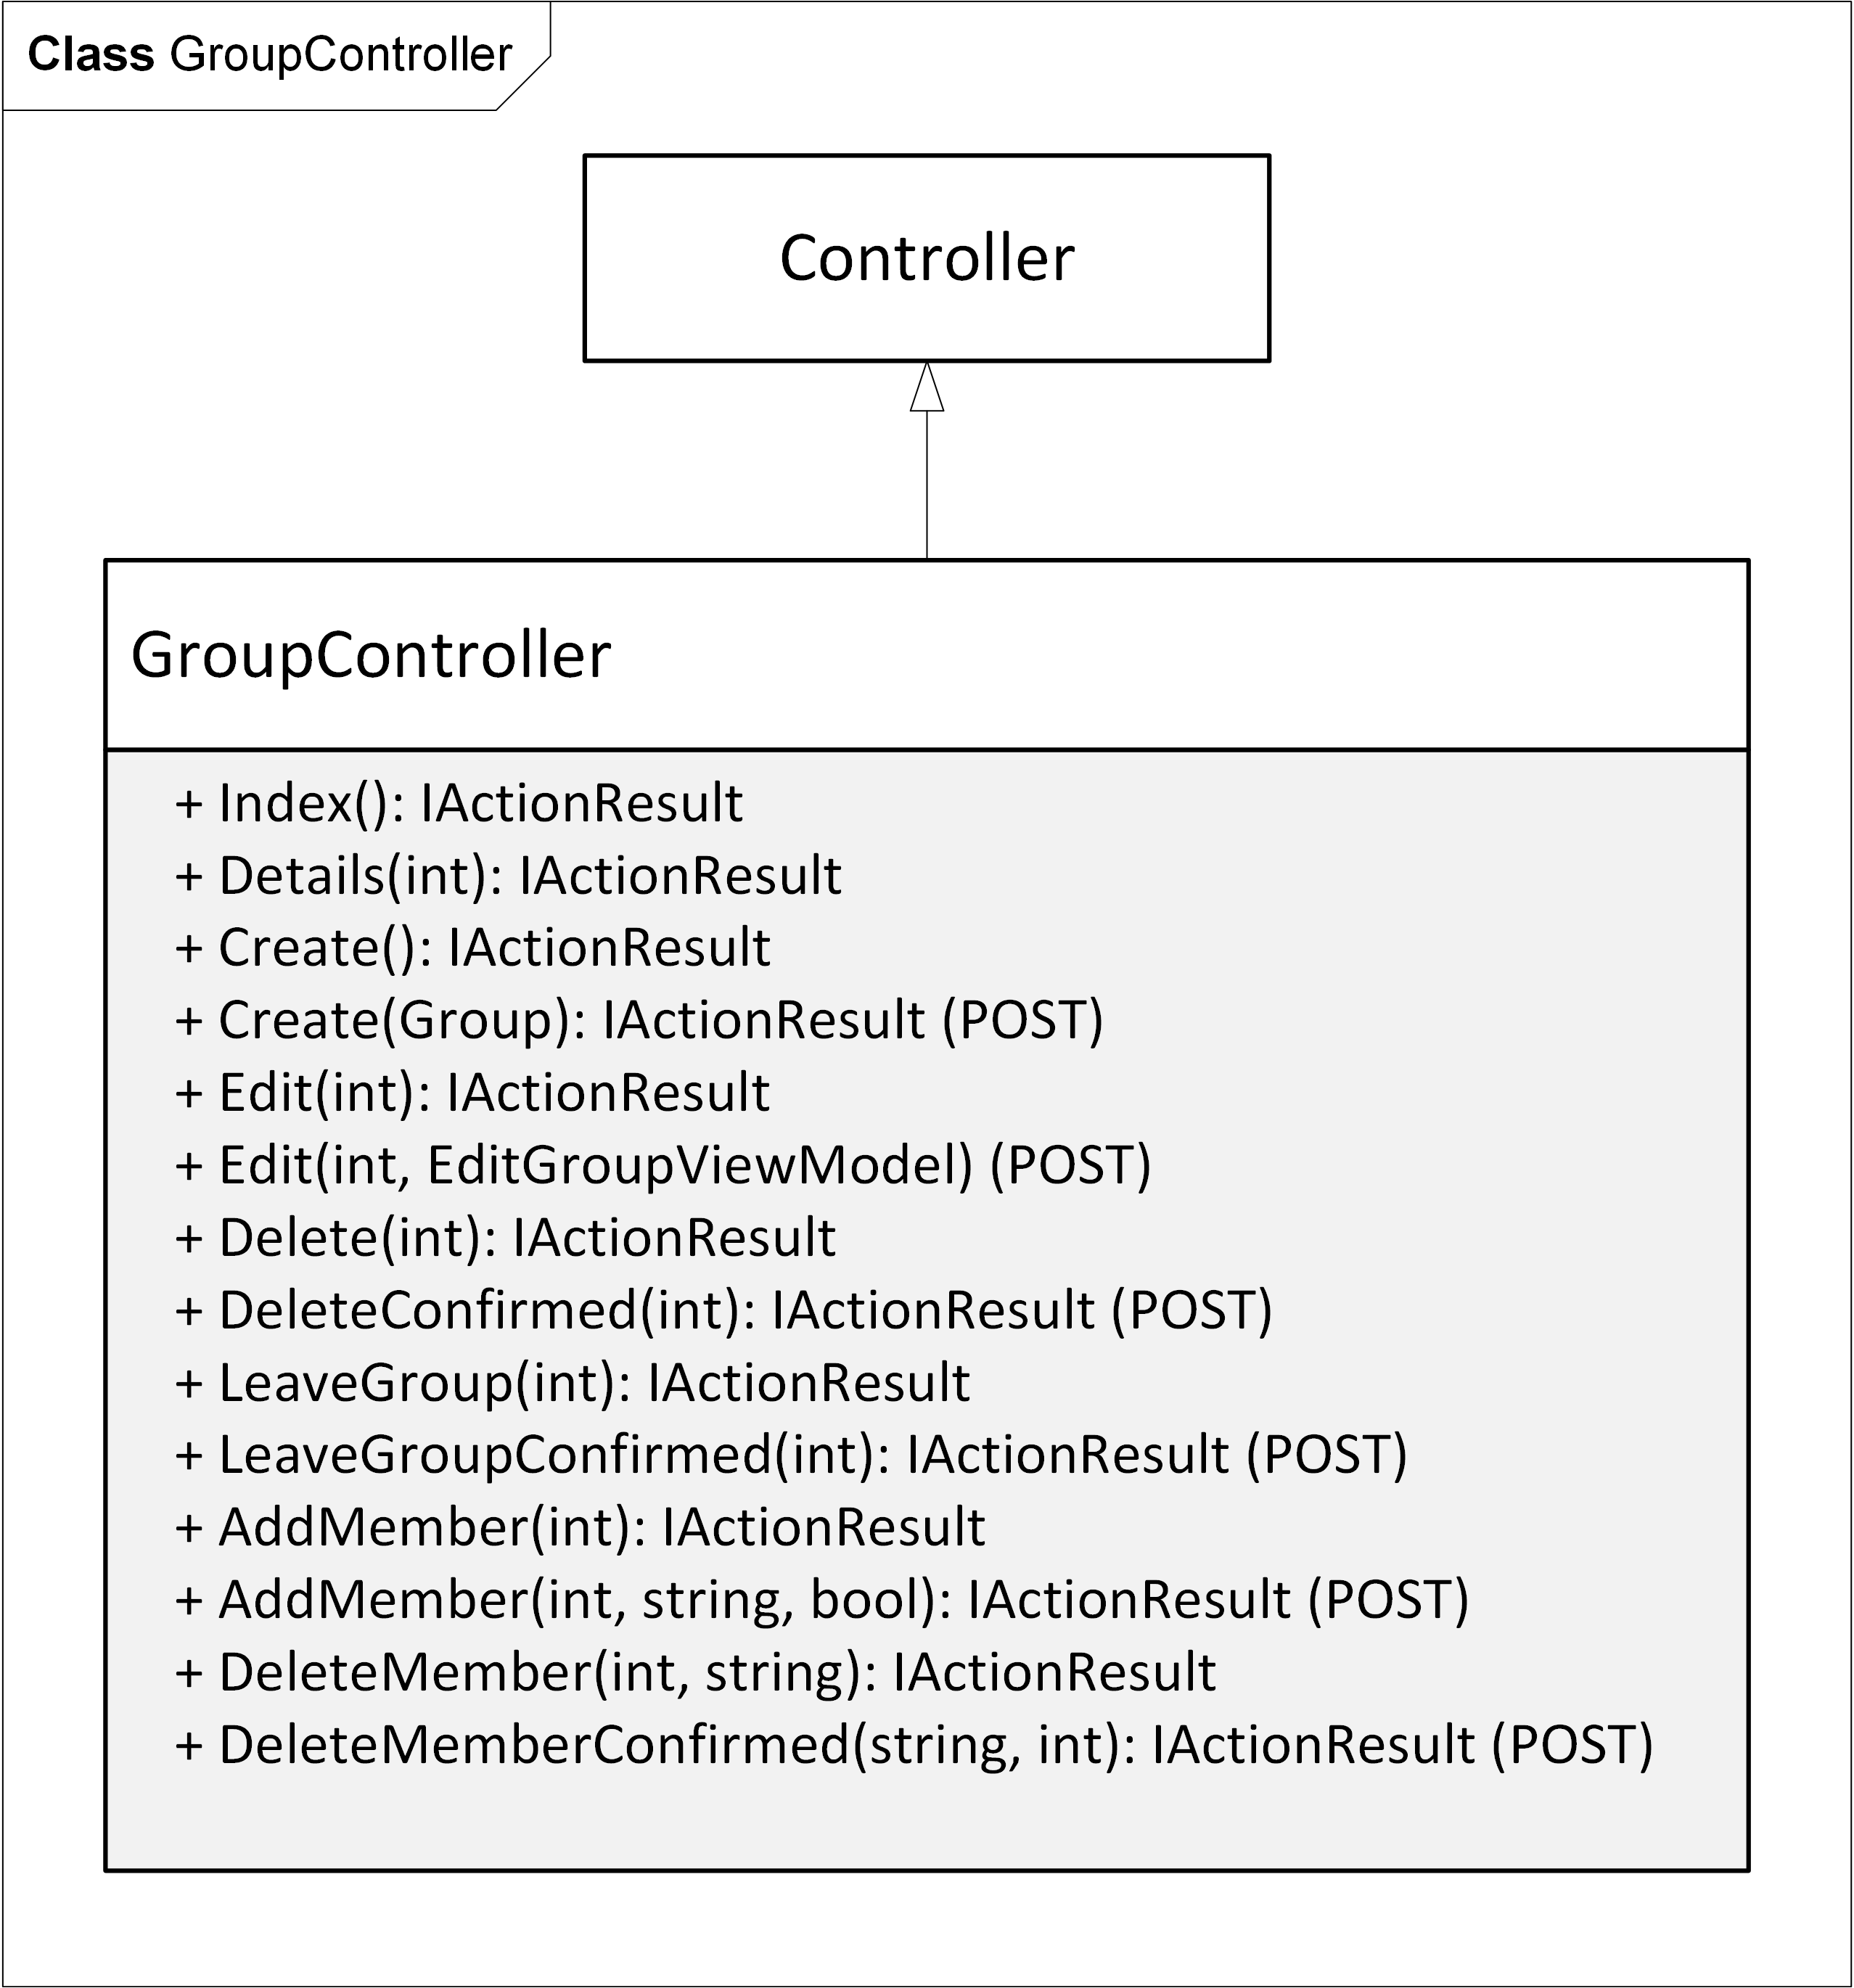
\includegraphics[scale=0.8]{01_Billeder/09_Arkitektur/Group/LogicalView_Class.png}
  \centering
  \caption{Klassediagram af GroupController. Funktioner hvor der står "POST" ud for, er en post funktion for den funktion som står lige over}
  \label{fig:group_logical_class}
\end{figure}

I bilag \thomas{henvisning} ses samme fremgangsmåde brugt på alle US's, som er blevet brugt til at fremstille det samlet klasse diagram for GroupController klassen på figur \ref{fig:group_logical_class}.